\section{Denotations}\label{sec:denote}

\subsection{Observation Variables}

Our program language is built upon basic atomic state-change
actions that modify global shared state $s$.
The concurrent flow of control is managed using a global label-set $ls$
and the association of two distinguished labels $in$ and $out$,
and a label generator $g$ with every language construct.

A key feature of this UTP semantics is that we have a key distinction
between two groups of observations that we wish to make of a running program.
\begin{description}
  \item[Dynamic State]~\\
    Both the global shared state and control-flow label-set
    are observations that change as the program executes.
    So our UTP theory will need to record both before- and after-values
    for both of these.
    \RLEQNS{
       s, s' &:& State        & \elabel{obs-s}
    \\ ls, ls' &:& \power Lbl & \elabel{obs-ls}
    }
  \item[Static Parameters]~\\
    The labels and generators associated with any given program
    construct are fixed during the lifetime of the program.
    They are determined statically by the context of each construct.
    For this reason we do not distinguish between before- and after-values
    \RLEQNS{
       in, out &:& Lbl & \elabel{obs-in-out}
    \\ g &:& Gen       & \elabel{obs-g}
    }
\end{description}
So our UTP theory has alphabet
\[
  \alpha P  = \setof{s,s',ls,ls',in,out,g}
  \qquad
  \elabel{alpha-P}
\]
and hence is based on a non-homogeneous relation.
This will not turn out to be problematical because
the formulation of the theory as described below will largely isolate the
two classes of observations.





\subsection{``Standard'' UTP Predicates}

Given a non-homogeneous alphabet,
some care has to be taken to define standard notions
from UTP theories, such as sequential composition ($\seq$),
and its unit predicate Skip $\Skip$.
The important thing here turns out to be that these concepts
completely ignore the static parameters.
So the definition of standard sequential composition
defines a mid-point state based solely on $s$ and $ls$:
\RLEQNS{
   P \seq Q
   &\defs& \exists s_m,ls_m \bullet
\\ && \qquad P[s_m,ls_m/s',ls'] \land Q[s_m,ls_m/s,ls]
   & \elabel{UTP-seq-def}
}
Similarly, $\Skip$, the behaviour that immediately terminates
without changing any state, only refers to the dynamic observations:
\RLEQNS{
   \Skip
   &\defs&
   s'= s \land ls'=ls
   & \elabel{UTP-skip-def}
}
It is easy to show that $\Skip$ is both a left- and right-unit for $\seq$.
\RLEQNS{
 \Skip \seq P &=~P~=& P \seq \Skip & \elabel{seq-unit}
}
Given the definitions above,
then the definitions of UTP conditionals and iteration
are quite standard.
\RLEQNS{
   P \cond C Q
   &\defs&
   C \land P \lor \lnot C \land Q
   & \elabel{UTP-cond-def}
\\ C * P
   &=&
   P ; C * P \cond C \Skip
   & \elabel{UTP-loop-unroll}
}
For iteration we juts present the loop unrolling law, as the most useful here.

We also define a specialised form of sequential composition
to be used when neither component refers to $ls$ or $ls'$,
and its unit $ii$:
\RLEQNS{
   P \seq_s Q
   &\defs&
   \exists s_m \bullet P[s_m/s'] \land Q[s_m/s]
   & \elabel{UTP-s-seq-def}
\\ ii &\defs& s'=s & \elabel{ii-def}
\\ ii \seq_s a \quad=& a &=\quad a \seq_s ii & \elabel{seq-s-unit}
}
Note that if neither predicate mentions $ls$ or $ls'$
then the effect of $\seq$ and $\seq_s$ is the same.
We often omit the $s$ subscript when its use is clear from context.

\subsubsection{Ground Expressions}

We assume a general notion of expressions ($e$)
and say that an expression $e$ is ``ground''
if its free variables are limited to only $g$, $in$ and $out$.
We say that a predicate is ground if all constituent expressions
are ground.
\RLEQNS{
   isGnd(e) &\defs&  FV(e) \subseteq \setof{g,in,out}
   & \elabel{gnd-expr-def}
\\ isGnd(P) &\defs&  FV(P) \subseteq \setof{g,in,out}
   & \elabel{gnd-pred-def}
}
This means that ground expressions in this setting can only
define either generators, label-sets, or atomic predicates
over these.
Indeed, generator expressions are ground by construction,
because the only variable they contain is precisely $g$.
It also means that a ground expression can always be simplified
to either a generator expression, enumerated label-set,
and any ground predicate to either true (valid) or false (a contradiction).

Substitution of expressions for free variables is
an important mechanism used to construct and reason about
UTP theories.
We define a substitution as being ground if the expressions
are all ground, and the target variables belong to $g$, $in$ and $out$.
\RLEQNS{
   isGnd[G,I,O/g,in,out] &\defs& isGnd(G) \land isGnd(I) \land isGnd(O)
   &\elabel{gnd-subs-def}
}
where $G$ is a generator expression,
and $I$ and $O$ are label-set expressions.
In the sequel we shall always assume that $G$, $I$ and $O$
stand for ground expressions, as here.

We shall use $\gamma$ to denote a ground substitution.
\RLEQNS{
  \gamma &=& [G,I,O/g,in,out] &\elabel{gamma-def}
}
The identity substitution can be written as a ground substitution:
\RLEQNS{
  \gamma_{id} &=& [g,in,out/g,in,out] & \elabel{gamma-id-def}
}

The significance of ground substitutions
is that they ignore UTP sequential composition,
in that they distribute through them,
and have no effect on Skip
\RLEQNS{
   (P\seq Q)\gamma &=& P\gamma \seq Q\gamma  & \elabel{seq-gnd-distr}
\\ \Skip\gamma     &=& \Skip                 &\elabel{skip-gamma}
}
They also distribute nicely through our invariant shorthands
\RLEQNS{
   ~\{L_1|\dots|L_n\}\gamma &=& \{L_1\gamma|\dots|L_n\gamma\}
   & \elabel{DL-gamma-subst}
\\ ~[L_1|\dots|L_n]\gamma &=& [L_1\gamma|\dots|L_n\gamma]
   & \elabel{LE-gamma-subst}
}

In addition, the set of all ground substitutions
is closed under substitution composition.
\RLEQNS{
  \exists G,I,O
  &@&
  [G_1,I_1,O_1/g,in,out] [G_2,I_2,O_2/g,in,out]
  =
   [G,I,O/g,in,out]
\\  && \elabel{gnd-sub-closure}
}


\subsubsection{Sound Substitutions}

Unfortunately, there are ground substitutions
that can break the unique label properties
we have worked so hard to achieve with our label generators.
A good example of this is $[g,\ell_g,\ell_g/g,in,out]$,
which can transform an invariant respecting predicate $P$
into one that violates that invariant in a strong way.

A ground substitution $[G,I,O/g,in,out]$ is sound
if the disjoint label invariant $\setof{I|G|O}$ is true.
\RLEQNS{
   isSound[G,I,O/g,in,out] &\defs& \setof{I|G|O}
   & \elabel{sound-sub-def}
}
We shall use $\varsigma$ to denote a sound substitution
\RLEQNS{
   \varsigma &=& [G,I,O/g,in,out] \textbf{ where } \setof{I|G|O} &\elabel{vsigma-def}
}
Note that $\gamma_{id}$ is sound.

All the substitutions explicitly given in the semantic rules below
are sound.
So it is particularly important that soundness is preserved by
substitution composition
\RLEQNS{
   isSound(\varsigma_1)
   \land
   isSound(\varsigma_2)
   &\implies&
   isSound(\varsigma_1\varsigma_2)
   & \elabel{sound-sub-closure}
}




\subsection{Healthiness Conditions}

\subsubsection{Disjoint Labels}

We have a general healthiness condition (Disjoint Labels) which asserts
that the labels associated with $in$, $out$ and $g$
are different:
\RLEQNS{
  \DL(P) &=& P \land \setof{in|g|out}
}
This is just the Disjoint Labels invariant of \S\ref{sssec:disjoint-labels},
reformulated as a healthiness condition.

\subsubsection{Wheels-within-Wheels}

The key intuition behind this compositional semantics was to take the
$run$ function of the action-system based semantic model used in UTPP,
and drive it inwards to every level of the program.
The original $run$ can be defined in the context of this theory as
\[
  run(P) = ls := \setof{in} ; \lnot (out \in ls) * P
\]
However this failed to keep atomic components ``live''.
They could never be re-executed,
as would be required if they were within an iteration.
Instead it was realised that every construct (atomic and composite)
would have to be within an infinite loop.
\RLEQNS{
   \W(P) &\defs& \true * P &\elabel{W-as-loop}
}
This bold step turns out to be remarkably effective,
with some quite counter-intuitive outcomes.
However it does depend on a specific tweak to the
definition of an atomic action.
In effect we define an atomic action
as placing a basic action inside such a loop,
but within a non-deterministic choice between it
and a \emph{stuttering} step, denoted by UTP skip:
\RLEQNS{
  \catom a &\defs& \W(\Skip \lor A(in|a|out))
}
A result of this is that this stuttering step gets
propagated up to enclosing composites,
so in effect we see $\W(C)=\W(\Skip\lor C)$
where $C$ is any predicate denoting the semantics of a command.
We give more details about this in the section on calculation (\S\ref{sec:calc}).
One key calculational advantage of this is that we can rewrite
the rhs of the definition of $\W$ as:
\RLEQNS{
   \W(P) &  =  & \bigvee_{i \in 0,\dots} \Skip \seq P^i &\elabel{W-as-NDC}
}%
We note explicitly here that, in effect,
our semantic model is based on unbounded non-determinism.

However, for iteration-free programs
we find that there is a finite $k$ such that $P^k = \false$,
in which case the non-determinism is bounded.
We get these finite results that seem very similar
to the results obtained by using $run$ above.
Using $run$ results in predicates that cannot be composed
to get composite behaviour.
However, using $\W$ results in a slight variation,
which is composable!
What turns out to be crucial
to this outcome is the explicit stuttering option in the infinite loop.


\subsection{UTP Denotational Semantics}

INTRODUCE

We present each construct individually,
with full diagrams for each \dots



\subsubsection{Basic Action}

Basic Action $A(E|a|N)$ is enabled when all the labels in $E$
are present in the global label-set
and atomic action $a$ does not evaluate to $\false$
in the current program state.
If so enabled,  it performs action $a$, removes the labels in $E$
from the label-set, and adds in those in $N$.
\RLEQNS{
   A(E|a|N)
   &\defs&
   ls(E) \land a \land ls'=(ls\setminus E) \cup N
   & \elabel{A-def}
}


We define what it means for an atomic action invocation
to satisfy an invariant parameterised on the label type ($Lbl$).
\RLEQNS{
  ls \textbf{ lsat } I \land A(E|a|N) &\implies& ls' \textbf{ lsat } I
}
We can re-formulate this as a following equivalent test:
\RLEQNS{
   A(E|a|N) \textbf{ sat } I_{Lbl}
   &\defs&
   E \textbf{ lsat } I_{Lbl} \land N \textbf{ lsat } I_{Lbl}
}

\RLEQNS{
   ls(\ell) &\defs& \ell \in ls
\\ ls(L) &\defs& L \subseteq ls
\\ ls(\B\ell) &\defs& \ell \notin ls
\\ ls(\B L) &\defs& L \cap ls = \emptyset
}


\newpage
\subsubsection{Atomic Action}

\includegraphics{images/atomic-action}
\RLEQNS{
  \catom a
  &\defs& \DL(\W(\Skip \lor A(in|a|out))) & \elabel{sem:atomic}
\\ &=&  [in|out] \land (\Skip \lor A(in|a|out))
        & \elabel{nf-atomic}
}

Invariant Preservation:
\RLEQNS{
   [in|out]\gamma \land A(in|a|out)\gamma &\implies& [in|out]'\gamma
   & \elabel{atom-inv-ok}
}

\subsubsection{Guarded Atomic Action}
In effect there is no real difference between $c \pgrd a$
and $\true \pgrd (c \land a)$,
so in fact we don't need guarded actions as basic.
This is an advantage of treating the atomic action as a relational predicate
on state.

\RLEQNS{
 c \pgrd a &\defs& \catom{c \land a}  &\elabel{sem:pgrd}
}


\subsubsection{Skip}

\RLEQNS{
   ii     &\defs& s'=s
\\ \cskip &\defs& \catom{ii}  &\elabel{sem:skip}
\\  &=&  [in|out] \land (\Skip \lor A(in|ii|out))
    &\elabel{nf-skip}
}

\newpage
\subsubsection{Sequential Composition}

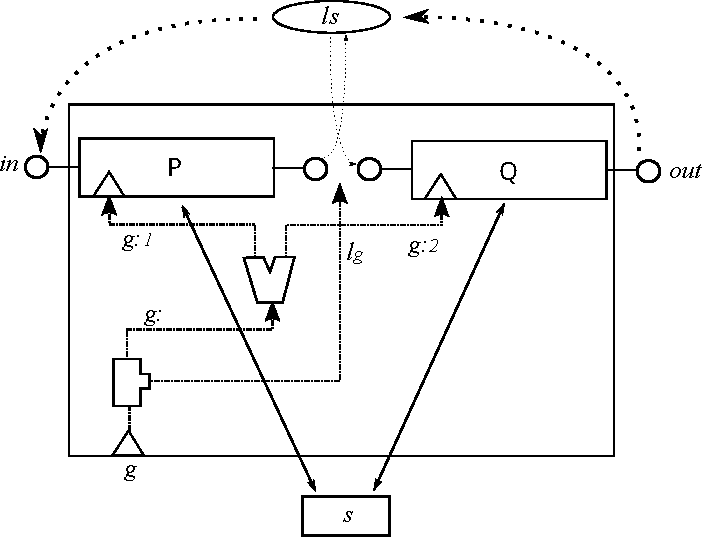
\includegraphics{images/seq-comp-actual}

\RLEQNS{
   P \cseq Q
   &\defs&
   [in|\ell_g|out]\land \W(P[g_{:1},\ell_g/g,out] \lor Q[g_{:2},\ell_g/g,in])
   & \elabel{sem:seq}
}

If $A$ actions in $P$ and $Q$ preserve the invariant,
then so does their composition.
This is immediate by the ground/sound substitution independence
of invariant preservation.



\newpage
\subsubsection{Parallel Composition}

\RLEQNS{
   P \parallel Q
   &\defs&
   [in|(\ell_{g1}|\ell_{g1:}),(\ell_{g2}|\ell_{g2:})|out] \land {}
   & \elabel{sem:par}
\\&& \W(\quad\phlor A(in|ii|\ell_{g1},\ell_{g2})
\\ && \qquad {}\lor
   P[g_{1::},\ell_{g1},\ell_{g1:}/g,in,out]
\\ && \qquad {}\lor
    Q[g_{2::},\ell_{g2},\ell_{g2:}/g,in,out]
\\ && \qquad {}\lor
   A(\ell_{g1:},\ell_{g2:}|ii|out)~)
}

\includegraphics{images/parallel-label-gen}

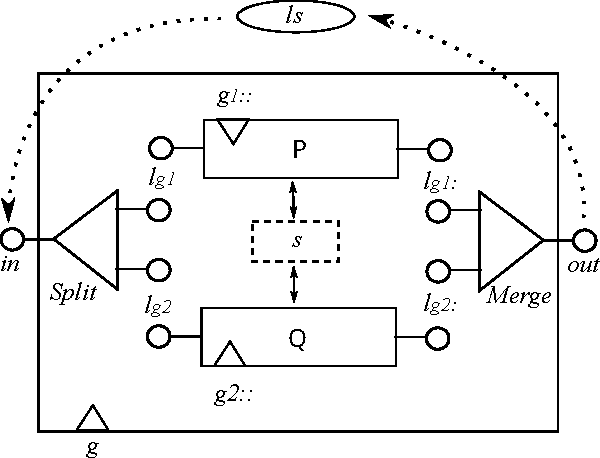
\includegraphics{images/par-comp-actual}


\newpage
\subsubsection{Nondeterministic Choice}

\RLEQNS{
   P + Q
   &\defs&
   [in|\ell_{g1}|\ell_{g2}|out] \land {}
   & \elabel{sem:NDC}
\\ && \W(\quad {}\phlor A(in|ii|\ell_{g1})
\\ && \qquad {} \lor
                     A(in|ii|\ell_{g2})
\\ && \qquad {} \lor
   P[g_{1:},\ell_{g1}/g,in]
\\ && \qquad {} \lor
   Q[g_{2:},\ell_{g2}/g,in]~)
}

\subsubsection{Nondeterministic Loop}


\RLEQNS{
   P^*
   &\defs&
   [in|\ell_g|out] \land {}
   & \elabel{sem:star}
\\ && \W(\quad  \phlor A(in|ii|out)
\\ && \qquad {}\lor A(in|ii|\ell_g)
\\ && \qquad {}\lor P[g_{:},\ell_g,in/g,in,out]~)
}

\newpage
\subsubsection{Conditional Choice}

\RLEQNS{
   P \dcond c Q
   &\defs&
   [in|\ell_{g1}|\ell_{g2}|out] \land {}
   & \elabel{sem:cond}
\\ && \W(\quad {}\phlor A(in|c \land ii|\ell_{g1})
\\ && \qquad {} \lor
                     A(in|\lnot c \land ii|\ell_{g2})
\\ && \qquad {} \lor
   P[g_{1:},\ell_{g1}/g,in]
\\ && \qquad {} \lor
   Q[g_{2:},\ell_{g2}/g,in]~)
}

\includegraphics{images/conditional-actual}

\newpage
\subsubsection{Conditional Loop}


\RLEQNS{
   c \ddo P
   &\defs&
   [in|\ell_g|out] \land {}
   & \elabel{sem:iter}
\\ && \W(\quad  \phlor A(in|\lnot c \land ii|out)
\\ && \qquad {}\lor A(in|c \land ii|\ell_g)
\\ && \qquad {}\lor P[g_{:},\ell_g,in/g,in,out]~)
}

\includegraphics{images/iteration-actual}

\newpage
\subsection{Essential Properties?}

The first key property is that every instance of $A$
in the semantics preserves the invariant.

Looking forward we will want some key algebraic properties:
\RLEQNS{
   A(E|a|N)\gamma &=& A(E\gamma|a|N\gamma)
\\ A(E|a|N) \textbf{ sat } I
   &=&
   A(E|a|N)\gamma \textbf{ sat } I\gamma
   , \quad \mbox{arbitrary }\gamma
\\ ((ls\setminus R)\cup A)(S)
   &=&
   ls(F(R,A,S)) \land P(R,A,S)
\\ \W(P)  && \textrm{monotonic in } P
\\ \W(\W(P)) &=& \W(P) & ?
\\ \W(\W(\Skip \lor P)) &=& \W(\Skip \lor P)
\\ \W(\Skip \lor P) &=& \bigvee_{i \in 0,\dots} \Skip \seq P^i
   & \elabel{W-as-NDC}
\\ \W(P)\gamma &=& \W(P\gamma) & \elabel{W-gamma-subst}
\\ \W(\Skip \lor P) &=& \Skip \lor \W(\Skip \lor P)
\\ I \land \W(P) &=& \W(I \land P) & \elabel{I-W-distr}
}


When $P\gamma$ executes:
\begin{description}
  \item[\elabel{P-removes-in}]
    it will remove $in\gamma$ from $ls$ at some point;
  \item[\elabel{P-removes-g}]
    the only other labels it removes are in $labs(g\gamma)$;
  \item[\elabel{P-adds-out}]
    it adds $out\gamma$ into $ls$ at some point;
  \item[\elabel{P-adds-g}]
    the only other labels it adds are in $labs(g\gamma)$;
  \item[\elabel{P-ignores-rest}]
    and its behaviour is not affected by any label not
    in
    \\$\setof{in\gamma,out\gamma} \cup labs(g\gamma)$.
\end{description}
We can summarise this as follows:
\begin{itemize}
  \item $P\gamma$ actions are enabled by labels in $in\gamma,g\gamma$
  \item $P\gamma$ actions enable actions enabled by $g\gamma,out\gamma$
  \item Remember that the following invariant holds: $[in\gamma|g\gamma|out\gamma]$
\end{itemize}




\newpage
\subsection{Miscellaneous}

Most of this stuff should end up,
if required,
in a Proofs/Justification appendix.

\subsubsection{Semantic Substitutions List}

It can be informative to see the invariants grouped with
the relevant actions and substitutions.
\RLEQNS{
   ~[in|out]
   && A(in|a|out)
\\ && id
\\
\\ ~[in|\ell_g|out]
   && [g_{:1},\ell_g/g,out]
\\ && [g_{:2},\ell_g/g,in]
\\
\\ ~[in|(\ell_{g1}|\ell_{g1:}),(\ell_{g2}|\ell_{g2:})|out]
   && A(in|ii|\ell_{g1},\ell_{g2})
\\ && A(\ell_{g1:},\ell_{g2:}|ii|out)
\\ && [g_{1::},\ell_{g1},\ell_{g1:}/g,in,out]
\\ && [g_{2::},\ell_{g2},\ell_{g2:}/g,in,out]
\\
\\ ~[in|\ell_{g1}|\ell_{g2}|out]
   && A(in|ii|\ell_{g1})
\\ && A(in|ii|\ell_{g2})
\\ && [g_{1:},\ell_{g1}/g,in]
\\ && [g_{2:},\ell_{g2}/g,in]
\\
\\ ~[in|\ell_g|out]
   && A(in|ii|out)
\\ && A(in|ii|\ell_g)
\\ && P[g_{:},\ell_g,in/g,in,out]
\\
\\ ~[in|\ell_{g1}|\ell_{g2}|out]
   && A(in|c \land ii|\ell_{g1})
\\ && A(in|\lnot c \land ii|\ell_{g2})
\\ && [g_{1:},\ell_{g1}/g,in]
\\ && [g_{2:},\ell_{g2}/g,in]
\\
\\ ~[in|\ell_g|out]
\\ && A(in|\lnot c \land ii|out)
\\ && A(in|c \land ii|\ell_g)
\\ && [g_{:},\ell_g,in/g,in,out]
}

\subsubsection{Nested Invariants}

For each composite,
we show how its component substitutions affect their invariants
and any entailment relationships that arise.
We don't show the conditional variants of choice and iteration
because their invariants and substitutions are the same as those
in the corresponding non-deterministic constructs.

Semantics Reminder:
\RLEQNS{
  \catom a
  &\defs& [in|out] \land \W(\Skip \lor A(in|a|out))
\\ P \cseq Q
   &\defs&
   [in|\ell_g|out]\land \W(P[g_{:1},\ell_g/g,out] \lor Q[g_{:2},\ell_g/g,in])
\\ P \parallel Q
   &\defs&
   [in|(\ell_{g1}|\ell_{g1:}),(\ell_{g2}|\ell_{g2:})|out] \land {}
\\&& \W(\quad\phlor A(in|ii|\ell_{g1},\ell_{g2})
\\ && \qquad {}\lor
   P[g_{1::},\ell_{g1},\ell_{g1:}/g,in,out]
\\ && \qquad {}\lor
    Q[g_{2::},\ell_{g2},\ell_{g2:}/g,in,out]
\\ && \qquad {}\lor
   A(\ell_{g1:},\ell_{g2:}|ii|out)~)
\\ P + Q
   &\defs&
   [in|\ell_{g1}|\ell_{g2}|out] \land {}
\\ && \W(\quad {}\phlor A(in|ii|\ell_{g1})
\\ && \qquad {} \lor
                     A(in|ii|\ell_{g2})
\\ && \qquad {} \lor
   P[g_{1:},\ell_{g1}/g,in]
\\ && \qquad {} \lor
   Q[g_{2:},\ell_{g2}/g,in]~)
\\ P^*
   &\defs&
   [in|\ell_g|out] \land {}
\\ && \W(\quad  \phlor A(in|ii|out)
\\ && \qquad {}\lor A(in|ii|\ell_g)
\\ && \qquad {}\lor P[g_{:},\ell_g,in/g,in,out]~)
}


\paragraph{Sequential Composition}

\begin{description}
  \item[Invariant]
    $[in|\ell_g|out]$
  \item[Substitutions]
    $[g_{:1},\ell_g/g,out]$ and $[g_{:2},\ell_g/g,in]$
  \item[Component Invariants]
    $$\begin{array}{|l|c|c|}
    \hline
      \mbox{Type} & \mbox{as }P & \mbox{as }Q
    \\\hline
      \catom\_ & [in|\ell_g] & [\ell_g|out]
    \\\hline
       \_\cseq\_& [in|\ell_{g:1}|\ell_g] & [\ell_g|\ell_{g:2}|out]
    \\\hline
       \_\parallel\_
       & [in|(\ell_{g:11}|\ell_{g:11:}),(\ell_{g:12}|\ell_{g:12:})|\ell_g]
       & [\ell_g|(\ell_{g:21}|\ell_{g:21:}),(\ell_{g:22}|\ell_{g:22:})|out]
    \\\hline
    \end{array}$$
\end{description}
Hmmm \dots, no simple relationship is emerging.
